\section{Combinatorial manifolds}

\begin{comment}

We will use two types of classical combinatorial structures: \emph{abstract polytopes} and \emph{combinatorial manifolds}. The latter is a subtype of the former. Abstract polytopes (or just ``polytopes'' in this note) encompass polygons, polyhedra, and higher-dimensional versions. They exclude certain undesirable shapes such as two triangles that meet at one vertex. But they aren't necessarily simplicial either:

\end{comment}


\begin{comment}
\subsection{Polytopes}

\begin{mydef}
A \defemph{finite abstract polytope} \( \mathcal{P} \) of dimension \( n \) is a finite poset \( P \) equipped with 
\begin{itemize}
\item two elements \( p_{\mathrm{min}}, p_{\mathrm{max}}:P \)
\item a \emph{rank} function \( r:P\to \zz \)
\end{itemize}
and properties
\begin{itemize}
\item a proof that \( a\leq b\to r(a)\leq r(b) \)
\item a proof that \( p_{\mathrm{min}} \) is minimal: \( \pit{p:P}p\geq p_{\mathrm{min}} \)
\item a proof that \( p_{\mathrm{max}} \) is maximal: \( \pit{p:P}p\leq p_{\mathrm{max}} \)
\item a proof that \( r(p_{\mathrm{min}}) = -1 \) (so that non-minimal elements have rank at least 0)
\item a proof that \( r(p_{\mathrm{max}}) = n+1 \) (so that non-maximal elements have rank at most \( n \))
\item a proof that rank ``counts containment'': \( \pit{a,b:P}(a\leq b)\times (\mathsf{is\_empty}\sit{c:P}(a\leq c\leq b))\to b=a+1 \)
\item a proof of \emph{strong connectedness} (all intervals are connected via a chain of containment): \newline\( \pit{a,b:P\setminus\{p_{\mathrm{min}}, p_{\mathrm{max}}\}}\left(\sit{x:P}a\leq x\leq b\text{ is connected}\right) \)
\item a proof of the \emph{diamond condition} that between two elements that differ by two ranks lie exactly two elements: \( \pit{a,b:P}(r(b)-r(a)=2)\to \#(\sit{c:P}a\leq c\leq b)=4 \) (of which \( a \) and \( b \) are two).
\end{itemize}
\end{mydef}

The diamond condition captures that two edges meet at a vertex, two faces meet at one edge, and so on. See the Hasse diagram (a graph of the poset with rank represented on the \( y \)-axis) of a tetrahedron in Figure~\ref{fig:hasse_tetrahedron} and the square pyramid (which will arise later as an octahedron minus its south pole) in Figure~\ref{fig:hasse_pyramid}.

\begin{figure}[htbp]
\centering
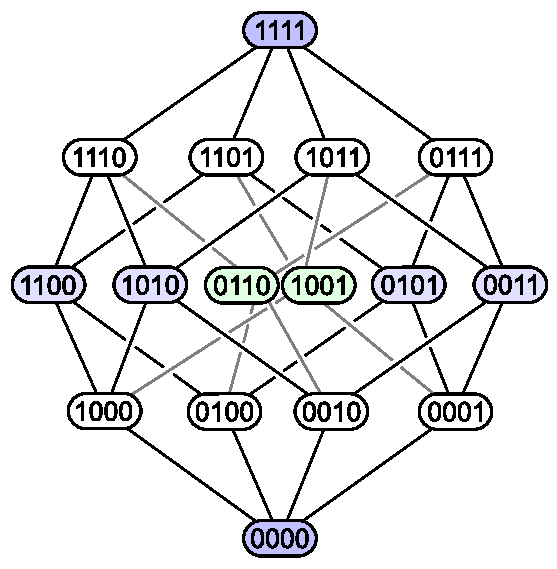
\includegraphics[width=200pt]{hasse_tetrahedron.pdf}
\caption{A finite abstract polytope representation of a tetrahedron, in the form of its ``Hasse diagram'' (from polytope.miraheze.org, public domain).}
\label{fig:hasse_tetrahedron}
\end{figure}

\begin{figure}[htbp]
\centering
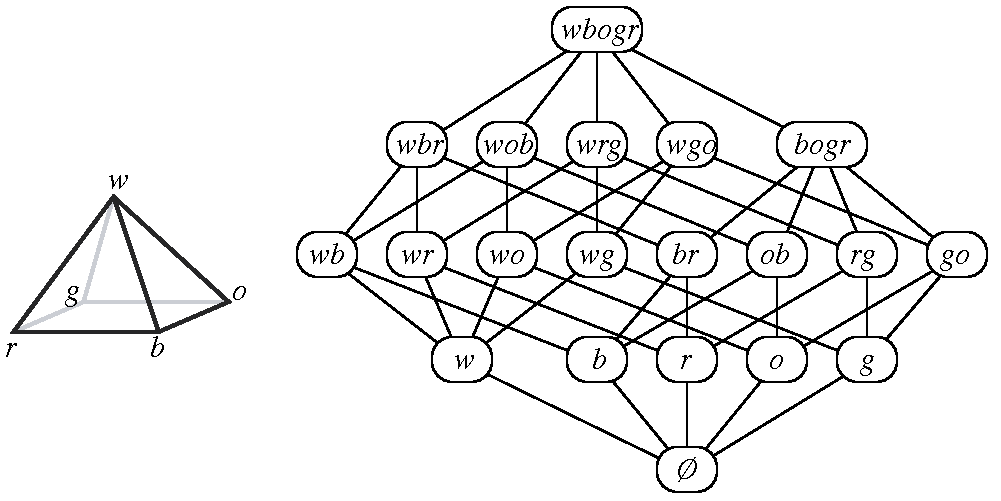
\includegraphics[width=350pt]{pyramid.pdf}
\caption{The Hasse diagram of a square pyramid (from wikimedia.org, public domain).}
\label{fig:hasse_pyramid}
\end{figure}

Next we will map abstract polytopes to higher inductive types. The poset structure will generate the paths, so the rank will correspond to the dimension. But as usual in a HIT we will need to make a choice of direction for each path constructor, which wasn't necessary in the polytope setting. We will restrict to dimension at most 2.

\begin{mydef}
A \defemph{higher inductive polytope (HIP) of dimension at most 2} \( \P \) for a polytope \( \mathcal{P} \) of dimension at most 2 is a type with constructor data given by
\begin{enumerate}
\item For each rank 0 element \( v \) a term \( V:\P \).
\item For each rank 1 element \( e \) and rank 1 pair \( v_1,v_2\leq e \) (cardinality 2 by the diamond condition) a path \( E:V_1=V_2 \).
\item For each rank 2 element \( f \) containing edges \( e_1,\ldots,e_n \) containing a cycle of vertex pairs \( \{\{v_{11},v_{12}\},\ldots,\{v_{n1},v_{n2}=v_{11}\}\} \) a 2-path \( F:E_1\cdot\ldots\cdot E_n=\refl_{v_{11}} \).
\end{enumerate}
\end{mydef}

\begin{mydef}
Given a HIT of dimension at most 2 we have the \defemph{skeleta} \( \P_0,\P_1,\P_2 \) where \( \P_i \) is the HIT generated by using the constructors up to dimension \( i \). The HIT also provides a chain of inclusions of skeleta \( \P_0\to\P_1\to\P_2 \).
\end{mydef}

If \( Z:\uni \) is a type then to define a map \( \P\to Z \) we start with a map \( \P\to Z \) and extend it to \( \P_1 \) and then \( \P_2 \). 


\end{comment}

\subsection{Combinatorial manifolds}

We will adapt to higher inductive types in a straightforward manner the classical construction of \emph{combinatorial manifolds}. See for example the classic book by Kirby and Siebenmann\cite{kirby_siebenmann}. These are a subclass of simplicial complexes.

\begin{mydef}
An \defemph{abstract simplicial complex \( M \) of dimension \( n \)} consists of a set \( M_0 \) of vertices, and for each \( 0<k\leq n \) a set \( M_k \) of subsets of \( M_0 \) of cardinality \( k+1 \), such that any \( (j+1) \)-element subset of \( M_k \) is an element of \( M_j \). The elements of \( M_k \) are called \defemph{\( k \)-faces}. Denote by \( \simcomp \) the type of abstract simplicial complexes of dimension \( n \) (where the suffix \( \mathsf{Set} \) reminds us that this is a type of sets).
\end{mydef}

Note that we don't require all subsets of \( M_0 \) to be included -- that would make \( M \) an individual simplex. A simplicial complex is a family of simplices that are identified along various faces.

\begin{mydef}
In an abstract simplicial complex \( M \) of dimension \( n \), the \defemph{link} of a vertex \( v \) is the \( n-1 \)-face containing every face \( m\in M_{n-1} \) such that \( v\notin m \) and \( m\cup v \) is an \( n \)-face of \( M \).
\end{mydef}

The link is all the neighboring vertices of \( v \) and the codimension 1 faces joining those to each other. See for example Figure~\ref{fig:link}.

\begin{figure}[htbp]
\centering
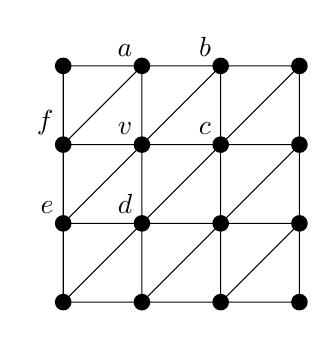
\begin{tikzpicture}
  \draw
    (0, 0) grid[step=1cm] (3, 3)
    (0, 2) -- (1, 3)
    (0, 1) -- (2, 3)
    (0, 0) -- (3, 3)
    (1, 0) -- (3, 2)
    (2, 0) -- (3, 1)
  ;
  \fill[radius=3pt]
    \foreach \x in {0, ..., 3} {
      \foreach \y in {0, ..., 3} {
        (\x, \y) circle[]
      }
    }
  ;
  \path[above left]
    \foreach \p/\v in {
      {1, 3}/a,
      {2, 3}/b,
      {0, 2}/f,
      {1, 2}/v,
      {2, 2}/c,
      {0, 1}/e,
      {1, 1}/d%
    } {
      (\p) node {$\v$}
    }
  ;
\end{tikzpicture}
\caption{The link of \( v \) in this complex consists of the vertices \( \{a,b,c,d,e,f\} \) and the edges \( \{ab,bc,cd,de,ef,fa\} \), forming a hexagon.}
\label{fig:link}
\end{figure}

\begin{mydef}
A \defemph{combinatorial manifold} (or \defemph{combinatorial triangulation}) of dimension \( n \) is a simplicial complex of dimension \( n \) such that the link of every vertex is a simplicial sphere of dimension \( n-1 \) (i.e. its geometric realization is homeomorphic to an \( n-1 \)-sphere). Denote by \( \combmfdset \) the type of combinatorial manifolds of dimension \( n \) (which the notation again reminds us are sets).
\end{mydef}

In a 2-dimensional combinatorial manifold the link is a polygon. See Figures~\ref{fig:sphere_triangulation}, \ref{fig:torus_wiki_triangulation}, and \ref{fig:genus3_wiki_triangulation} for some examples of 2-dimensional combinatorial manifolds of genus 0, 1, and 3.

A classical 1940 result of Whitehead, building on Cairn, states that every smooth manifold admits a combinatorial triangulation\cite{whitehead_triangulation}. So it appears reasonably well motivated to study this class of objects.

\begin{figure}[htbp]
\centering
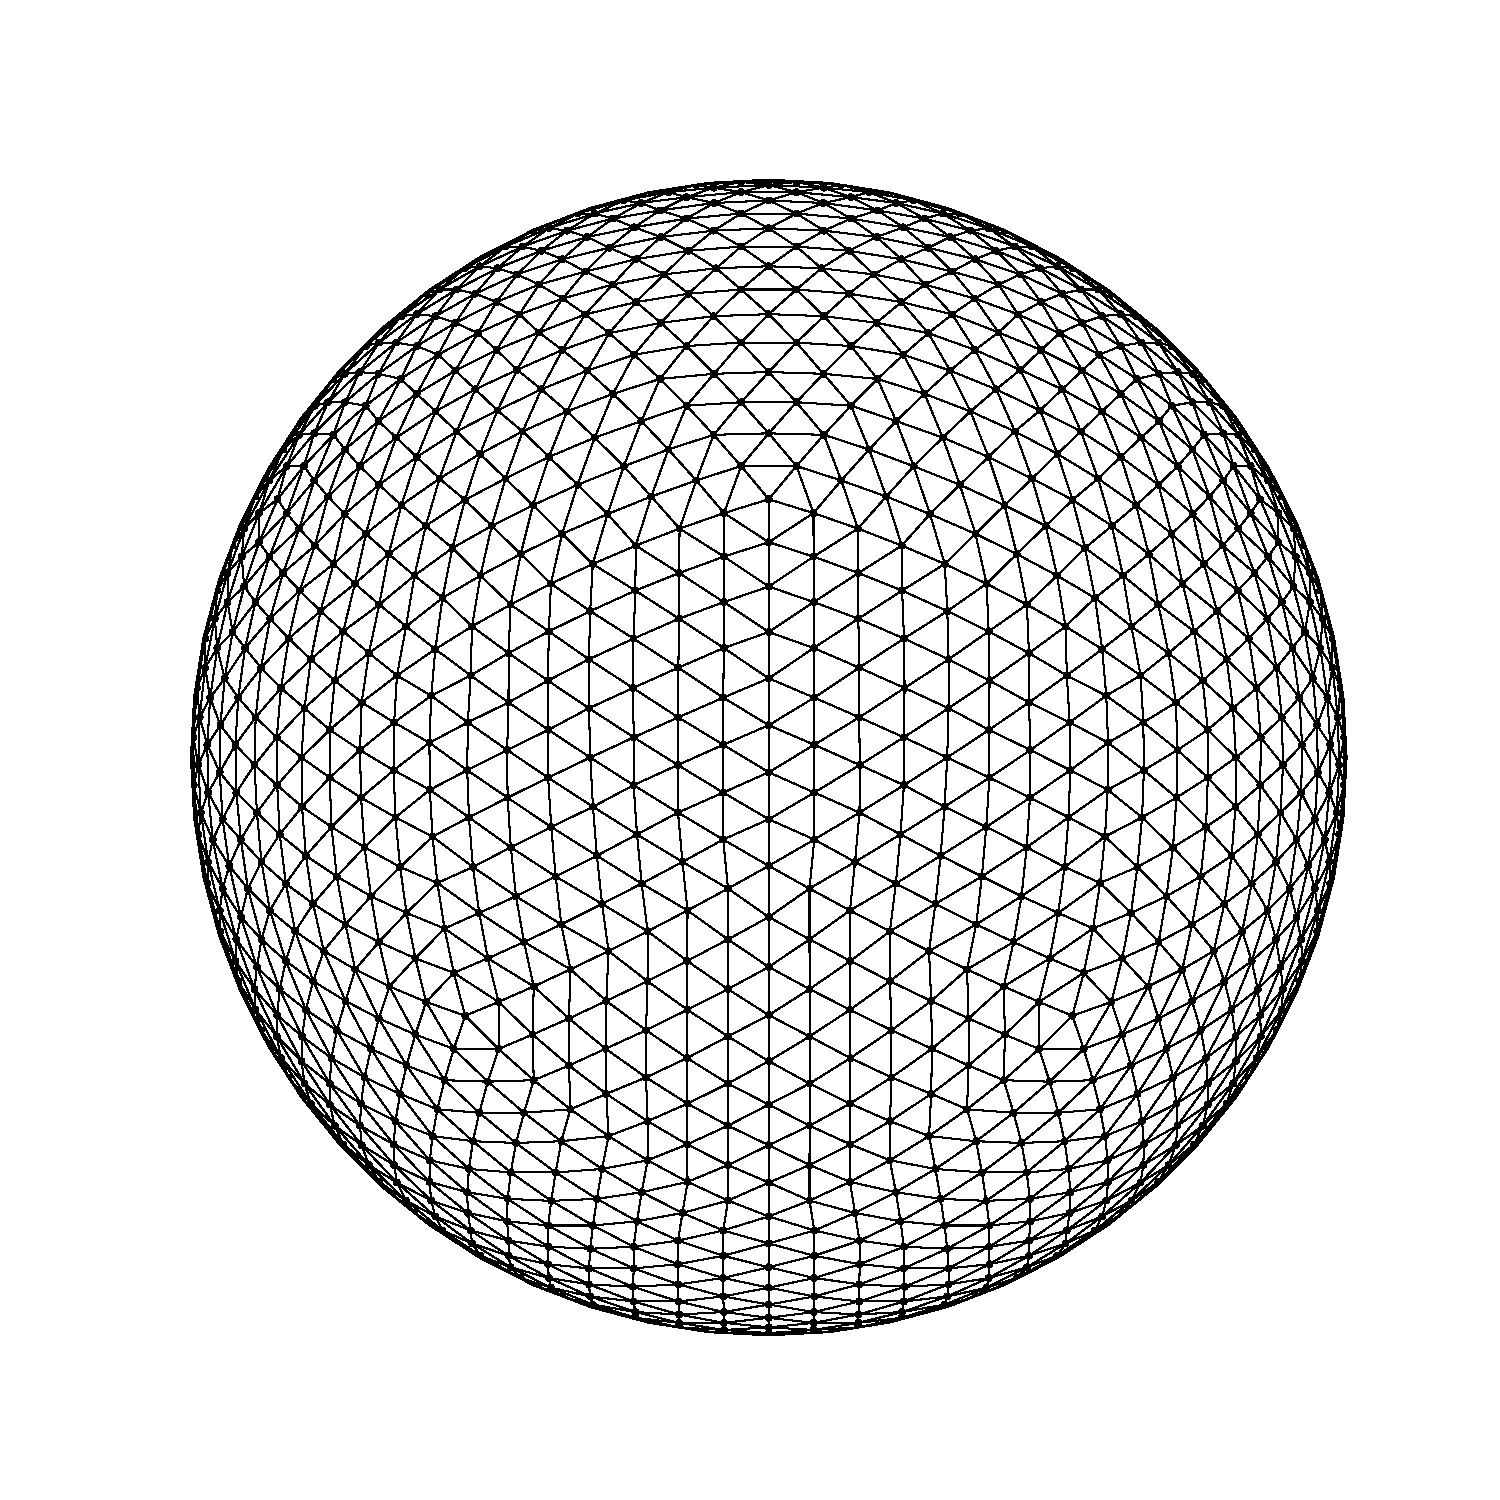
\includegraphics[width=200pt]{triangulated_sphere.pdf}
\caption{A combinatorial triangulation of a sphere, created with the tool \texttt{stripy}.}
\label{fig:sphere_triangulation}
\end{figure}

\begin{figure}[htbp]
\centering
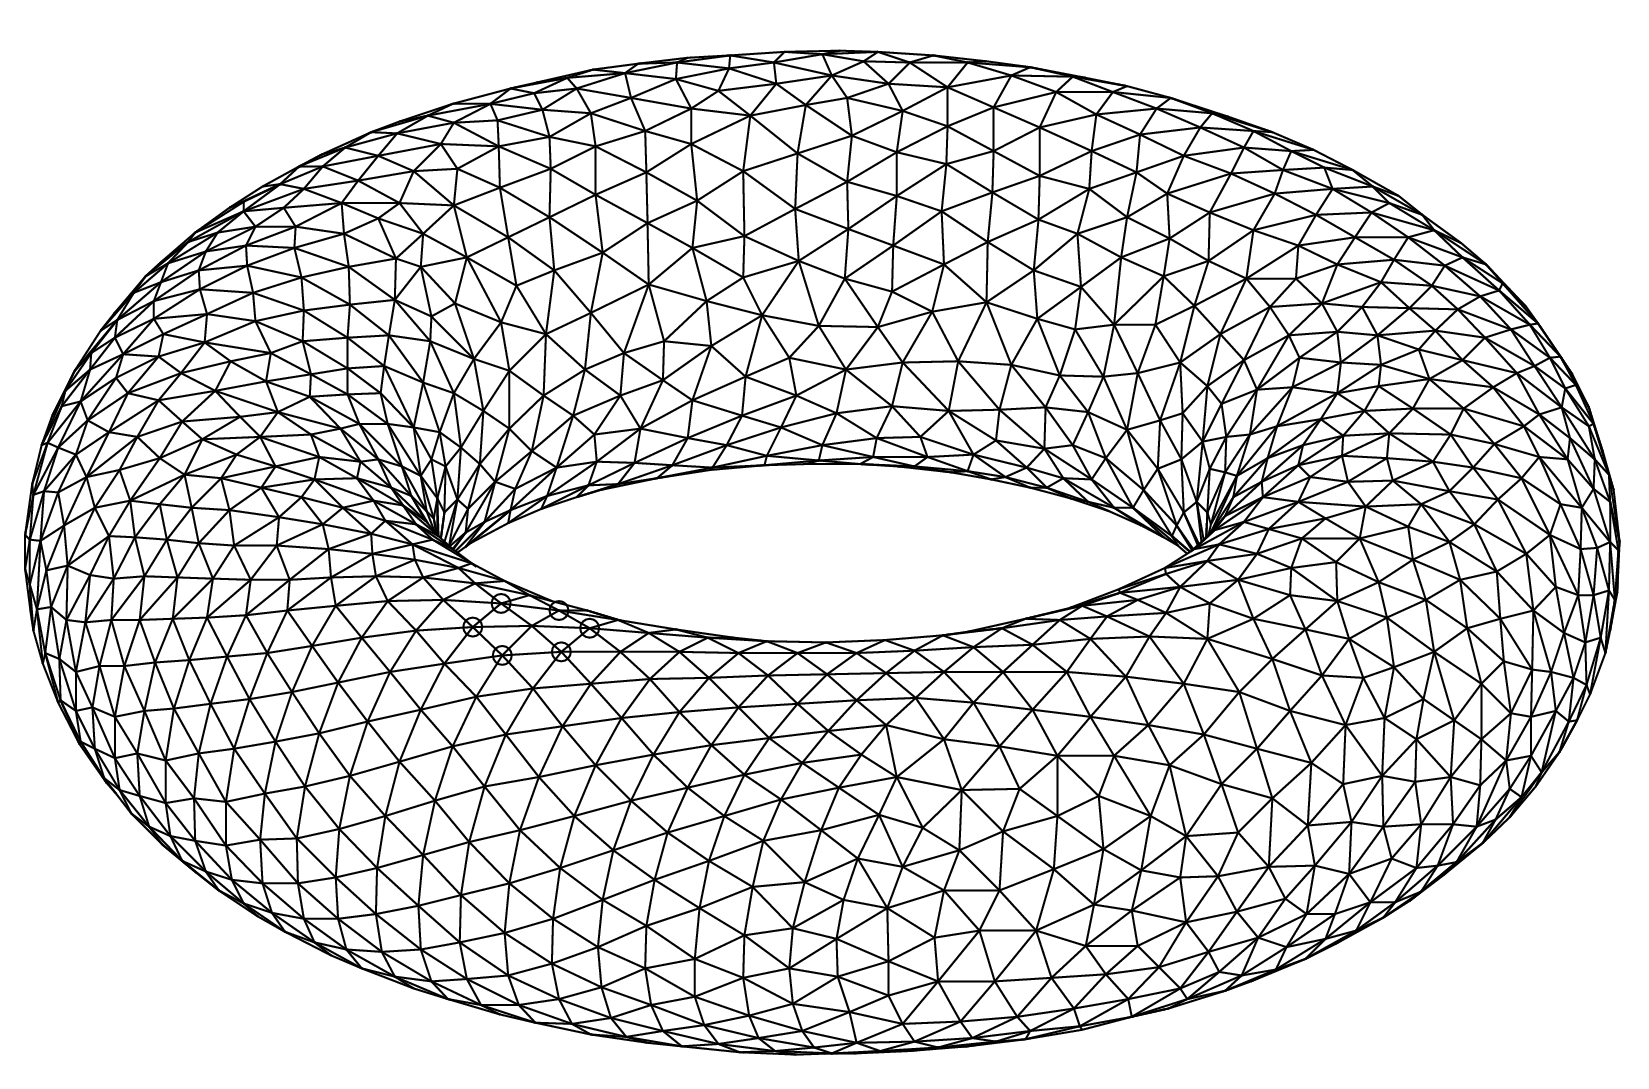
\includegraphics[width=200pt]{Torus-triang.png}
\caption{A torus with an interesting triangulation, from Wikipedia. The links have various vertex counts from 5-7. Clearly a constant value of 6 would also work. (\href{https://commons.wikimedia.org/w/index.php?curid=30856793}{By Ag2gaeh} - Own work, CC BY-SA 3.0.)}
\label{fig:torus_wiki_triangulation}
\end{figure}

\begin{figure}[htbp]
\centering
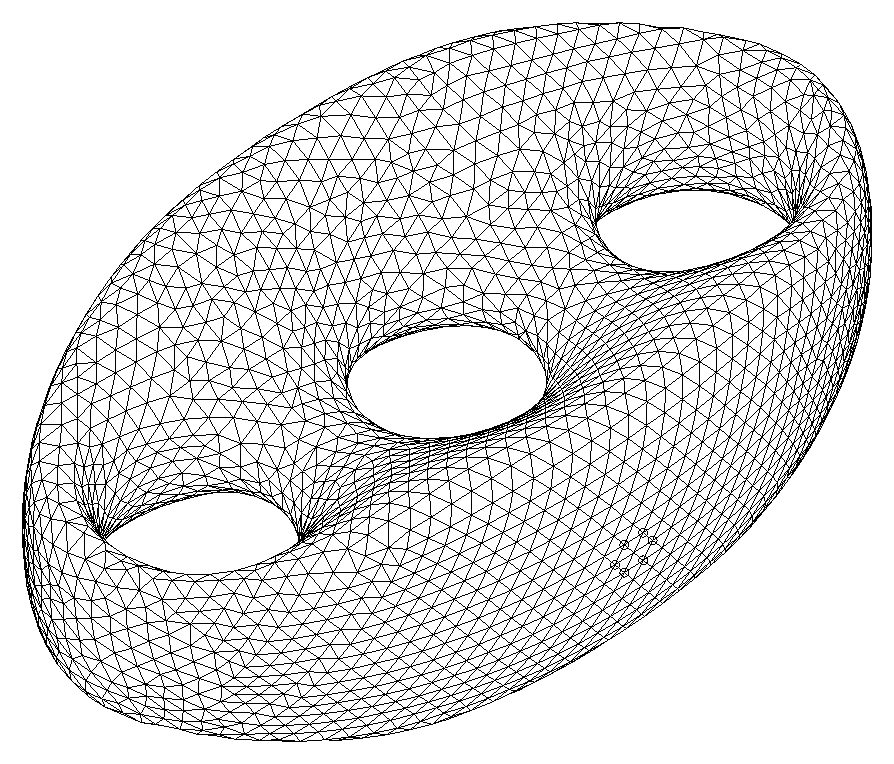
\includegraphics[width=200pt]{triangulated_genus3.pdf}
\caption{A 3-holed torus with triangulation, from Wikipedia. (\href{https://commons.wikimedia.org/wiki/File:Tri-brezel.svg}{By Ag2gaeh} - Own work, CC BY-SA 3.0.)}
\label{fig:genus3_wiki_triangulation}
\end{figure}

\subsection{Higher inductive combinatorial manifolds}

We will convert a simplicial complex \( M \) of dimension at most 2 to a higher inductive type, in two steps. 

\begin{mydef}
Define \( \combmfdt \) to be the type of \defemph{higher inductive constructors of combinatorial manifolds of dimension at most 2} and let \( \mathcal{H}:\combmfdsett\to\combmfdt \) be a map from a combinatorial manifold to such a HIT following this method:
\begin{enumerate}
\item vertices: a function \( \mathsf{v_0}:M_0\to \mathcal{H}(M) \) serving as the 0-dimensional constructors
\item edges: a function \( \mathsf{v_1} \) on 1-faces, sending \( \{a, b\}\mapsto \mathsf{v_0}(a)=\mathsf{v_0}(b) \)
\item 2-faces: a function \( \mathsf{v_2} \) on 2-faces, sending \( \{a, b, c\}\mapsto \refl_a = \mathsf{v_1}(\{a, b\})\cdot \mathsf{v_1}(\{b, c\})\cdot \mathsf{v_1}(\{a, c\})^{-1} \).
\end{enumerate}
\end{mydef}

We will assume there is a formal theory of such HITs, and that at least up to dimension 2 there are no obstructions to simply copying over the combinatorial data to the HIT constructors. For recent work on HITs see for example David Wärn's discussion of pushouts\cite{warn_pushouts}.

\begin{mydef}
Denote by \( \re:\combmfdt\to\Type \) the process of generating a type from the HIT data (which we refer to as \defemph{realization}). Note that \( \re(\mathcal{H}(M)) \) is not in general a set, and may not even be 2-truncated for an arbitrary 2-dimensional combinatorial manifold \( M:\combmfdsett \).
\end{mydef}

We're making the distinction between \( \mathcal{H} \) and \( \re \) because we will mostly study functions and phenomena on \( \mathcal{H}(M) \) for some simplicial complex \( M \).

\subsection{Polygons}\label{sec:polygons}

We will now start looking at some examples, first by defining a type that is important both for the domain and the codomain of mere circles: a square.

\begin{mydef}
The higher inductive type \( C_4 \) (where C stands for ``circle''). See Figure~\ref{fig:c4}.
\begin{align*}
C_4 &: \Type \\
c_1, c_2, c_3, c_4 &: C_4 \\
c_1c_2 &: c_1 = c_2 \\
c_2c_3 &: c_2 = c_3 \\
c_3c_4 &: c_3 = c_4 \\
c_4c_1 &: c_4 = c_1 \\
\end{align*}
\end{mydef}

\begin{figure}[htbp]
\centering
\begin{tikzpicture}[
node distance = 15mm and 15mm,
V/.style = {circle, fill, draw=black, inner sep=1pt, font=\footnotesize},
every edge quotes/.style = {auto, font=\footnotesize},
arrow/.style={->,semithick}
]
\begin{scope}[nodes=V]
  \node[label=above left:\( c_1 \)] (1) {};
  \node[label=above right:\( c_2 \)] (2) [right=of 1]  {};
  \node[label=below right:\( c_3 \)] (3) [below=of 2]  {};
  \node[label=below left:\( c_4 \)] (4) [below=of 1]  {};
\end{scope}
\draw[arrow]
        (1)  edge["\( c_1c_2 \)"] (2)
        (2)  edge["\( c_2c_3 \)"] (3)
        (3)  edge["\( c_3c_4 \)"] (4)
        (4)  edge["\( c_4c_1 \)"] (1);
\end{tikzpicture}

\caption{The HIT \( C_4 \).}
\label{fig:c4}
\end{figure}

The standard HoTT circle itself is a non-example of a combinatorial manifold since it lacks the second vertex of the edge:

\begin{mydef}
The higher inductive type \( \so \) which we can also call \( C_1 \):
\begin{align*}
\so &:\Type \\
\mathsf{base}&:\so \\
\mathsf{loop}&:\mathsf{base}=\mathsf{base}
\end{align*}
\end{mydef}

Both of these are examples of a family of HIT data we will call \( \Gon \), the type of \( n \)-gon HITs for some natural number \( n \), following the pattern of the HITs above. We'll see below that the realization of an \( n \)-gon is a mere circle, i.e. we have \( \re:\Gon\to \EMzo \).

\subsection{Adding and removing points from polygons}
Given functions \( \phi,\psi:A\to B \) between two arbitrary types we can form the type family of paths \( \alpha:A\to\uni, \alpha(a)\defeq(\phi(a)=_B\psi(a)) \). Transport in this family is given by concatenation as follows, where \( p:a=_A a' \) and \( q:\phi(a)=\psi(a) \) (see Figure~\ref{fig:transport_family_of_paths}):
\[ 
\tr(p)(q) = \phi(p)^{-1}\cdot q\cdot \psi(p)
\]
which gives a path in \( \phi(a')=\psi(a') \) by connecting dots between the terms \( \phi(a'), \phi(a), \psi(a), \psi(a') \). This relates a would-be homotopy \( \phi\sim\psi \) specified at a single point, to a point at the end of a path. We will use this to help construct such homotopies.

\begin{figure}[htbp]
\centering
\begin{tikzpicture}[
node distance = 20mm and 20mm,
V/.style = {circle, fill, draw=black, inner sep=1pt},
every edge quotes/.style = {auto},
arrow/.style={->,semithick}
]
\begin{scope}[nodes=V]
  \node[label=above left:\( \phi(a) \)] (1) {};
  \node[label=above right:\( \phi(a') \)] (2) [right=of 1]  {};
  \node[label=below right:\( \psi(a') \)] (3) [below=of 2]  {};
  \node[label=below left:\( \psi(a) \)] (4) [below=of 1]  {};
  \node[label=below:\( a \)] (5) [below=of 4]  {};
  \node[label=below:\( a' \)] (6) [below=of 3]  {};
\end{scope}
\draw[arrow]
        (2)  edge[swap, "\( \phi(p)^{-1} \)"] (1)
        (4)  edge["\( \psi(p) \)"] (3)
        (1)  edge[swap, "\( q \)"] (4)
        (5)  edge["\( p \)"] (6);
\end{tikzpicture}
\caption{Transport along \( p \) in the fibers of a family of paths. The fiber over \( a \) is \( \phi(a)=\psi(a) \) where \( \phi,\psi:A\to B \).}
\label{fig:transport_family_of_paths}
\end{figure}

\begin{mylemma}\label{lem:addpoints}
Let \( C_n \) be the polygon 1-dimensional HIT with \( n \) vertices. Then \( C_2\simeq C_1 \) and in fact \( C_n\simeq C_{n-1} \).
\end{mylemma}
\begin{proof}
(Compare to \cite{hottbook} Lemma 6.5.1.) In the case of \( C_1 \) we will denote its constructors by \( \base \) and \( \loopo \). For \( C_2 \) we will denote the points by \( v_1, v_2 \) and the edges by \( \ell_{12}, r_{21} \). For \( C_3 \) and higher we will denote the points by \( v_1,\ldots,v_n \) and the edges by \( e_{i,j}:v_i=v_j \) where \( j=i+1 \) except for \( e_{n,1} \). 

First we will define \( f:C_2\to C_1 \) and \( g:C_1\to C_2 \), then prove they are inverses.
\begin{align*}
f(v_1)=f(v_2)&=\base &\quad g(\base)&=v_1\\
f(\ell_{12})&=\loopo&\quad g(\loopo)&=\ell_{12}\cdot r_{21}\\
f(r_{21}) &= \refl_{\base}& & \\
\end{align*}

We need to show that \( f\circ g\sim \id_{C_1} \) and \( g\circ f\sim\id_{C_2} \).
Think of \( f \) as sliding \( v_2 \) along \( r_{21} \) to coalesce with \( v_1 \). This may help understand why the unfortunately intricate proof is working.

We need terms \( p:\pit{a:C_1}f(g(a))=a \) and \( q:\pit{a:C_2}g(f(a))=a \). We will proceed by induction, defining appropriate paths on point constructors and then checking a condition on path constructors that confirms that the built-in transport of these type families respects the definition on points.

Looking first at \( g\circ f \), which shrinks \( r_{21} \), we have the following data to work with:
\begin{align*}
g(f(v_1))=g(f(v_2))&=v_1\\
g(f(\ell_{12}))&=\ell_{12}\cdot r_{21}\\
g(f(r_{21})) &= \refl_{v_1}.
\end{align*}
We then need to supply a homotopy from this data to \( \id_{C_2} \), which consists of a section and pathovers over \( C_2 \):
\begin{align*}
p_1&:g(f(v_1))=v_1\\
p_2&:g(f(v_1))=v_2\\
H_\ell&:\tr(\ell_{12})(p_1)=p_2\\
H_r&:\tr(r_{21})(p_2)=p_1.
\end{align*}
which simplifies to
\begin{align*}
p_1&:v_1=v_1\\
p_2&:v_1=v_2\\
H_\ell&:g(f(\ell_{12}))^{-1}\cdot p_1\cdot \ell_{12}=p_2\\
H_r&:=g(f(r_{21}))^{-1}\cdot p_2\cdot r_{21}= p_1
\end{align*}
and then to 
\begin{align*}
p_1&:v_1=v_1\\
p_2&:v_1=v_2\\
H_\ell&:(\ell_{12}\cdot r_{21})^{-1}\cdot p_1\cdot \ell_{12}=p_2\\
H_r&:\refl_{v_1}\cdot p_2\cdot r_{21}= p_1
\end{align*}

To solve all of these constraints we can choose \( p_1\defeq\refl_{v_1} \), which by consulting either \( H_\ell \) or \( H_r \) requires that we take \( p_2\defeq{r_{21}}^{-1}\).

Now examining \( f\circ g \), we have
\begin{align*}
f(g(\base))&=\base&\\
f(g(\loopo))&=f(\ell_{12}\cdot r_{21})=\loopo
\end{align*}
and so we have an easy proof that this is the identity.

The proof of the more general case \( C_n \simeq C_{n-1}\) is very similar. Take the maps \( f:C_n\to C_{n-1} \), \( g:C_{n-1}\to C_n \) to be
\begin{align*}
f(v_i)=v_i&\quad(i=1,\ldots,n-1) & g(v_i)&=v_i&\quad(i=1,\ldots,n-1)\\
f(v_n)=v_1&\quad& g(e_{i,i+1})&=e_{i,i+1}&\quad(i=1,\ldots,n-2)\\
f(e_{i,i+1})=e_{i,i+1}&\quad(i=1,\ldots,n-1)& g(e_{n-1,1})&=e_{n-1,n}\cdot e_{n,1}&\\
f(e_{n-1,n})=e_{n-1,1}&&&&\\
f(e_{n,1})=\refl_{v_1}&&&&
\end{align*}
where \( f \) should be thought of as shrinking \( e_{n,1} \) so that \( v_n \) coalesces into \( v_1 \).

The proof that \( g\circ f\sim\id_{C_n} \) proceeds as follows: the composition is definitionally the identity except 
\begin{align*}
g(f(v_n))&=v_1\\
g(f(e_{n-1,n}))&=e_{n-1,n}\cdot e_{n,1}\\
g(f(e_{n,1}))&= \refl_{v_1}.
\end{align*}
Guided by our previous experience we choose \( {e_{n,1}}^{-1}:g(f(v_n))=v_n \), and define the pathovers by transport.

The proof that \( f\circ g\sim\id_{C_{n-1}} \) requires only noting that \( f(g(e_{n-1,1}))=f(e_{n-1,n}\cdot e_{n,1})=e_{n-1,1}\cdot\refl_{v_1}=e_{n-1,1} \).
\end{proof}

\begin{mycor}
All polygons are equivalent to \( \so \), i.e. we have a term in \( \pit{n:\nn}||C_n=S^1|| \), and hence \( \Gon \) is a subtype of \( \EMzo \).
\end{mycor}
\begin{proof}
We can add \( n-1 \) points to \( S^1 \) and use Lemma~\ref{lem:addpoints}.
\end{proof}

\begin{mydef}
For \( k:\nn \) define \( m_k:\Gon\to\Gon \) where \( m_k:C_n\to C_{kn} \) adds \( k \) vertices between each of the original verticies of \( C_n \).
\end{mydef}

With \( m_k \) we can start with a surface that has pentagonal plus hexagonal links, and apply \( m_6 \) to the pentagons and \( m_5 \) to the hexagons, and have a type family that is the tangent bundle (because it comes from the link) but where every fiber has 30 vertices.

\subsection{\texorpdfstring{The higher inductive type \( \oo \)}{The higher inductive type O}}

We will create our first combinatorial surface, a 2-sphere. We will adopt the convention that a subscript indicates the dimension of a subskeleton of a complex. For instance, we have \( \mathsf{base}:\so_0 \).

\begin{mydef}
The HIT \( \oo_0 \) is just 6 points, intended as the 0-skeleton of an octahedron, with vertices named after the colors on the faces of a famous Central European puzzle cube.
\[ w, y, b, r, g, o : \oo_0 \]
\end{mydef}

\begin{mydef}
The HIT \( \oo_1 \) is the 1-skeleton of an octahedron.
\begin{align*}
w, y, b, r, g, o &: \oo_1 & yg &: y=g \\
wb &: w=b & yo &: y=o \\
wr &: w=r & br &: b=r \\
wg &: w=g & rg &: r=g \\
wo &: w=o & go &: g=o \\
yb &: y=b & ob &: o=b \\
yr &: y=r
\end{align*}
\end{mydef}

\begin{mydef}
The HIT \( \oo \) is an octahedron:
\begin{align*}
w, y, b, r, g, o &: \oo \\
wb &: w=b & br &: b=r & wbr &: wb\cdot br\cdot wr^{-1} = \refl_w \\
wr &: w=r & rg &: r=g & wrg &: wr\cdot rg\cdot wg^{-1} = \refl_w \\
wg &: w=g & go &: g=o & wgo &: wg\cdot go\cdot wo^{-1} = \refl_w \\
wo &: w=o & ob &: o=b & wob &: wo\cdot ob\cdot wb^{-1} = \refl_w \\
yb &: y=b & & & yrb &: yr\cdot rb\cdot yb^{-1} = \refl_y \\
yr &: y=r & & & ygr &: yg\cdot gr\cdot yr^{-1} = \refl_y \\
yg &: y=g & & & yog &: yo\cdot og\cdot yg^{-1} = \refl_y \\
yo &: y=o & & & ybo &: yb\cdot bo\cdot yo^{-1} = \refl_y 
\end{align*}
\end{mydef}

\begin{figure}[htbp]
\centering
\begin{figure}[h]
\centering
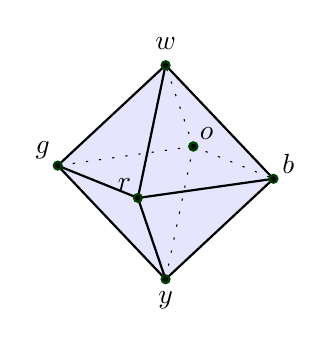
\begin{tikzpicture}%
  [x={(-0.860769cm, -0.121512cm)},
  y={(0.508996cm, -0.205391cm)},
  z={(-0.000053cm, 0.971107cm)},
  scale=1,
  back/.style={loosely dotted, thin},
  edge/.style={black, thick},
  facet/.style={fill=blue!95!black,fill opacity=0.1},
  vertex/.style={inner sep=1pt,circle,draw=green!25!black,fill=black,thick}]
\coordinate (-1, -1, 0) at (-1, -1, 0);
\coordinate (-1, 1, 0) at (-1, 1, 0);
\coordinate (0, 0, -1) at (0, 0, -1);
\coordinate (0, 0, 1) at (0, 0, 1);
\coordinate (1, -1, 0) at (1, -1, 0);
\coordinate (1, 1, 0) at (1, 1, 0);
%% Drawing edges in the back
%%
\draw[edge,back] (-1, -1, 0) -- (-1, 1, 0);
\draw[edge,back] (-1, -1, 0) -- (0, 0, -1.4);
\draw[edge,back] (-1, -1, 0) -- (0, 0, 1.4);
\draw[edge,back] (-1, -1, 0) -- (1, -1, 0);
%% Drawing vertices in the back
%%
\node[vertex] at (-1, -1, 0)     {};
%% Drawing the facets
%%
\fill[facet] (1, 1, 0) -- (0, 0, -1.4) -- (1, -1, 0) -- cycle {};
\fill[facet] (1, 1, 0) -- (0, 0, 1.4) -- (1, -1, 0) -- cycle {};
\fill[facet] (1, 1, 0) -- (-1, 1, 0) -- (0, 0, 1.4) -- cycle {};
\fill[facet] (1, 1, 0) -- (-1, 1, 0) -- (0, 0, -1.4) -- cycle {};
%% Drawing edges in the front
%%
\draw[edge] (-1, 1, 0) -- (0, 0, -1.4);
\draw[edge] (-1, 1, 0) -- (0, 0, 1.4);
\draw[edge] (-1, 1, 0) -- (1, 1, 0);
\draw[edge] (0, 0, -1.4) -- (1, -1, 0);
\draw[edge] (0, 0, -1.4) -- (1, 1, 0);
\draw[edge] (0, 0, 1.4) -- (1, -1, 0);
\draw[edge] (0, 0, 1.4) -- (1, 1, 0);
\draw[edge] (1, -1, 0) -- (1, 1, 0);
%% Drawing the vertices in the front
%%
\begin{scope}[nodes=vertex]
\node[label=above right:\( b \)] at (-1, 1, 0)     {};
\node[label=below:\( y \)] at (0, 0, -1.4)     {};
\node[label=above:\( w \)] at (0, 0, 1.4)     {};
\node[label=above left:\( g \)] at (1, -1, 0)     {};
\node[label=above left:\( r \)] at (1, 1, 0)     {};
\node[label=above right:\( o \)] at (-1, -1, 0)     {};
\end{scope}
\end{tikzpicture}
\caption{The HIT \( \oo \) which has 6 points, 12 1-paths, 8 2-paths.}
\end{figure}

\caption{The HIT \( \oo \) which has 6 points, 12 1-paths, 8 2-paths.}
\end{figure}

We have obvious maps \( \oo_0\xrightarrow[]{i_0} \oo_1\xrightarrow[]{i_1} \oo \) that include each skeleton into the next-higher-dimensional skeleton.
